\documentclass[12pt]{article}

\usepackage{graphicx}
\usepackage{color}
\usepackage[colorlinks]{hyperref}

\title{IDP alpha tutorial}
\author{Max Talanov}
\date{\today}

\begin{document}

\maketitle

\section{Outline}
\tableofcontents

\section{Overview}
IDP stands for intellectual document processing. IDP is capable of creating XML structures on base of simple texts and machine learning technique, in other words IDP is a project of machine learned structurisation and normalization of the unstructured text of natural language.\\
Actually this means that IDP is capable to split ordinary text on logical spans based on learned information during training by human process. Also it is possible to setup normalization rules to transform contents of some spans to place it in DB or valid XML.\\ 
IDP uses: \href{http://minorthird.sourceforge.net/}{minorthird} for natural language processing, \href{jgap.sourceforge.net}{JGAP} for normalization of English and Russian dates, \href{http://www.vistaicons.com/}{VISTAICO AERO PACK} for icon set.

\section{Start up}
This is short description of setup and installation process.
\begin{enumerate}
  \item You have to have Java version 6, please download from \href{http://java.sun.com/javase/downloads/index.jsp}{Sun microsystems site}
  \item Download client and server archives from \href{http://code.google.com/p/idp/downloads/list}{IDP download page} (You must have done this)
  \item Unzip client and server archives to separate directories ex.: \emph{server} and \emph{client} respectively
  \item Start server: in \emph{server} directory: under Windoz: run \emph{startServer.bat}, under Linux: run \emph{chmod +x startServer.sh} then \emph{./startServer.sh}. Though you can make some setup in properties file, I would recommend to stay on default settings at the moment.
  \item Start client: in \emph{client} directory: under Windoz: run \emph{startClient.bat}, under Linux: run \emph{chmod +x startClient.sh} then \emph{./startClient.sh}
\end{enumerate}
This is actually all what you need to do to start using IDP.\\
This is possible that there could be some errors in server or in client parts, please be patient and submit bug reports, if you find some.

\section{Client GUI}

\subsection{GUI areas}
Client GUI has several sections or areas shown on the picture below.\\
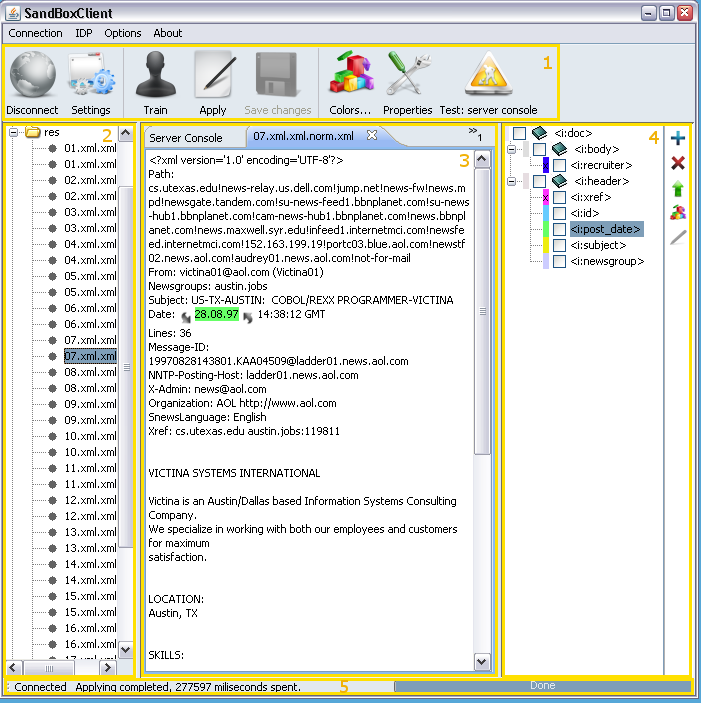
\includegraphics[scale=0.6]{00ClientAreas.png}
\begin{enumerate}
        \item Toolbar - mainly the server commands and settings.
	\item Project tree - directory structure of the project.
	\item Work panel - area for manual annotation and server console.
	\item Annotation tree - XML tree of annotated text.
	\item Status bar - Shows current state and progress of the commands.
\end{enumerate}

\subsection{Connect to the server}
When you start client you are able to do no so much: Setup server settings, connect to the server. Note status bar is indicating \emph{Not connected} state. First of all, please  connect to the server. Please press connect button 
\includegraphics[scale=0.6]{02ConnectButton.png}.\\
Connect button should change to Disconnect, and status bar should indicate \emph{Connected}.\\
In project tree, you should see \emph{example\_1} project name. Please expand \emph{example\_1}, double clacking on it. You should see \emph{apply} and \emph{train} directories.

\subsection{Upload files}
Please right click on \emph{train} directory and choose \emph{Upload...} item of menu, then choose three files from directory, where you have unpacked client archive, from \emph{example\_1/train} directory.\\
If files uploaded successfully, you should see \emph{File has been uploaded successfully!} message. Please upload all \emph{train} directory contents, this will more or less guarantee, correct training. Then upload 3-5 files to \emph{apply} directory from \emph{examle\_1/apply} directory of client archive, for example \texttt{01.txt}, \texttt{02.txt}, \texttt{03.txt}. You should be able to see all uploaded files in directory tree, please do not forget to expand directories \emph{apply} and \emph{train}.

\subsection{Train}
Train is done mainly automatically by the server. To train please click on Train button 
\includegraphics[scale=0.6]{03TrainButton.png}. Work panel should display a lot of messages and progress bar in lower left corner should display name of training stage and percent of completeness of training. When training is complete you should be able to see \emph{Training has been completed successfully!} message, progress bar should display \emph{Done} message.

\subsection{Apply with normalization}
This is mainly most complex operation for the server, and requires some significant time.\\
Please click on 
\includegraphics[scale=0.6]{04ApplyButton.png}.\\
First you should see a lot of messages in the server console and progress bar should indicate \emph{Loading annotators}, \emph{Annotating texts}, \emph{Normalising result xml files} stages. Please note that \emph{Normalization} should take time, because of Genetic Algorithms invoked in the process.\\
After all you should see \emph{Annotation has been completed successfully!} message and \emph{res} directory should emerge in project tree.

\subsection{View annotated texts}
Expand \emph{res} directory, double click on some file in \emph{res} directory, that ends with \emph{txt.xml}, but without \emph{norm.xml} at the end, ex.: \texttt{01.txt.xml}.
Work panel should display contents of xml file without xml tags. Annotation tree panel should display root element of xml tree result of annotation \emph{i:doc}.\\
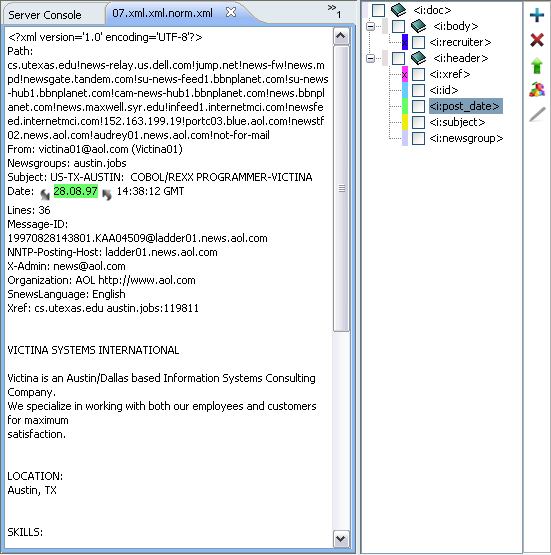
\includegraphics[scale=0.6]{05AnnotationPanel.png}

\subsubsection{Normalization}
Please double click on \emph{i:doc}, you should see tree drop down \emph{i:body} and \emph{i:header}, double click on \emph{i:header}, then select \emph{i:post\_date}.
Please double click on another file that ends with \emph{.norm.xml} but with same name to previously opened, ex.: \texttt{01.txt.xml.norm.xml}. Select \emph{i:post\_date}, you should be able to notice difference of representation of the date, for example in file \emph{01.txt.xml} \emph{i:post\_date} is \texttt{23 Aug 97} and in \emph{01.txt.xml.norm.xml} \texttt{23.08.97}. Actually this is result of normalization.\\

\subsubsection{Annotated text colors}
At the moment you should see curly arrows around \emph{post\_date} and value should be selected with color 
\includegraphics[scale=1.0]{06AnnotatedText.png}.\\
Please use toolbar button 
\includegraphics[scale=1.0]{07ChangeTagColor.png} \emph{Change tag color ...}  to setup color of selected tag.

\subsection{Change annotation and retrain}
Please open three \emph{txt.xml} files from \emph{res} directory. Select \emph{i:id} tag in \emph{Annotation tree} and expand annotation to include \texttt{\&gt;} or \texttt{\&lt;}. Please don't forget to press \emph{Save changes} 
\includegraphics[scale=0.6]{11SaveChanges.png} button every time you change annotation. \emph{corrected} directory with edited files should emerge in project tree. Please run \emph{Train} again, as described above. Note that at the end of \emph{Train} stage, you should be able to see corrected files in \emph{train} directory. Add not processed txt files from \emph{examle\_1/apply} directory of client archive, for example \texttt{18.txt}, \texttt{19.txt}, \texttt{20.txt}. Run \emph{Apply}. After all you should be able to see new files in \emph{res} directory. Please click on new files, you should see annotation of \emph{i:id} includes \texttt{\&gt;} 
\includegraphics[scale=1.0]{08CorrectedAnnotation.png}.

\subsection{New element in Annotation tree}
 Please close all opened tabs in work panel, delete all files from \emph{apply} directory, upload \emph{17.txt} file from client archive to \emph{apply} directory. Expand \emph{res} directory, open \texttt{18.txt.xml}, \texttt{19.txt.xml}, \texttt{20.txt.xml}, expand \emph{i:doc}, \emph{i:header} elements in \emph{Annotation tree}. Select \emph{i:header}, press 
\includegraphics{09AddAChildTag.png} button, set \emph{org} name of the tag. Do not forget to save changes, click 
\includegraphics[scale=1.0]{12UploadTreeChanges.png} in \emph{Annotation tree} panel. Expand tree back.\\

Select \emph{i:org} element of the tree. Press 
\includegraphics{10MarkTag.png} tool of \emph{Annotation tree} toolbar. Answer \emph{Ok} in pop-up dialog. Select text to the right of \emph{Organization:}, for example in \emph{20.txt.xml} it is \emph{New Resources Corporation}. Press \emph{Yes} in choose dialog to confirm your selection. Click on 
\includegraphics[scale=0.6]{11SaveChanges.png} button to save changes of each file. Run \emph{Train}, delete all files from \emph{res} directory, run Apply. Expand \emph{res} directory, open result file \emph{17.txt.xml}, note \emph{Annotation tree} contains \emph{i:org} element and it is annotated.\\
Close client.\\
To stop server please run in \emph{server} directory: under Windoz: \emph{stopServer.bat}, under Linux:\emph{chmod +x stopServer.sh} then \emph{stopServer.sh}.

\section{FAQ}
\begin{description}
	\item[Why is it client-server] - Because Server really needs fast machine with 1Gb of free memory, especially in case of other than Enlish languages.
        \item[Can I use it for not English] - Yes. IDP has been tested with Russian CV documents. We can not guarantee that it will really work on your documents (well it is still alpha).
        \item[What about integration with different systems] - Not yet. IDP produces XML files, and that's it at the moment.
        \item[Can I report a bug] - Yes please, use \href{http://code.google.com/p/idp/issues/list}{IDP issues list}.
        \item[Why is it alpha] - Because it has not really been tested on different datasets. We are sure, there are a lot of bugs. Please be patient.
        \item[Does your server really support multiple clients] - Not at the moment.
        \item[Can I use different to text and xml input files] - Not at the moment.
        \item[How many documents are ok to train] - Depends, train set should describe context of text to be annotated as completely as possible.
\end{description}

\end{document}
